\documentclass[11pt]{article}
\usepackage[a4paper,margin=1in]{geometry}
\usepackage{fontspec}
\usepackage{xeCJK}
\usepackage{graphicx}
\usepackage{booktabs}
\usepackage{caption}
\usepackage{parskip}

\setmainfont{Times New Roman}
\setsansfont{Arial}
\setCJKmainfont{Songti SC}
\setCJKsansfont{STHeiti}

\title{Traditional 与 Learning-based 事件表示简要对比报告}
\author{}
\date{2026-05-07}

\begin{document}
\sloppy
\maketitle

\paragraph{实验范围。} 当前仓库中可以用于汇报的结果覆盖三条主线：N-MNIST 分类、N-Caltech101 分类和 MVSEC optical flow。Traditional baseline 共包含 5 个方法：Event Frame、Binary Event Image、Timestamp Image、Time Surface 和 Voxel Grid。Learning-based 方面，N-MNIST 当前可见 EvRepSL 一个结果；N-Caltech101 包含 EST adaptation、EvRepSL、EST End-to-End、Event Pre-training、EventOrdering、GET 和 Matrix-LSTM；MVSEC 包含 EST、ERGO、GET、Event Pre-training、EvRepSL 和 MatrixLSTM。需要注意，分类任务中不同 learning-based 方法的实现栈并不完全相同；MVSEC 则是更严格的统一协议比较，所有方法共享同一个 EVFlowNet-like decoder 和相同 early stopping 设置。

\begin{figure}[t]
  \centering
  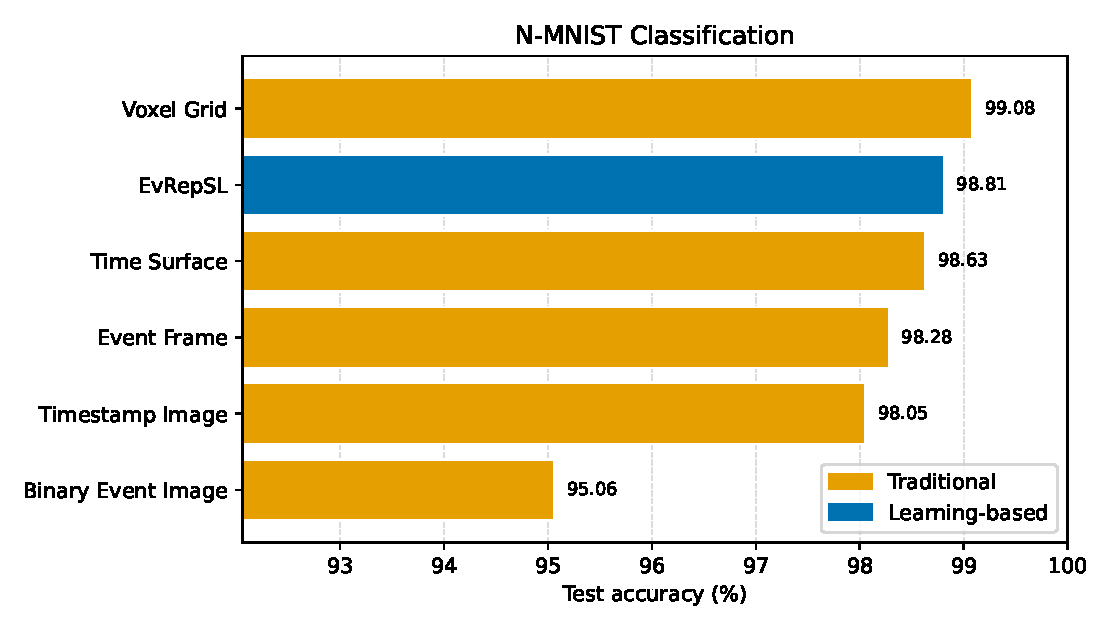
\includegraphics[width=0.86\linewidth]{nmnist_accuracy_brief.pdf}
  \caption{N-MNIST 分类准确率对比。当前仓库中 N-MNIST learning-based 只有 EvRepSL 一个结果，因此该图主要用于说明 N-MNIST 已接近饱和，而不是完整 learning-based suite 对比。}
  \label{fig:nmnist}
\end{figure}

\paragraph{N-MNIST：任务接近饱和，差距不宜过度解读。} 如图 \ref{fig:nmnist} 所示，N-MNIST 上大部分方法准确率都超过 98\%。Traditional 中 Voxel Grid 最高，达到 99.08\%；Learning-based 的 EvRepSL 为 98.81\%；Time Surface 为 98.63\%，Event Frame 为 98.28\%，Timestamp Image 为 98.05\%。Voxel Grid 与 EvRepSL 的差距只有 0.27 个百分点，说明当前 N-MNIST 结果更多反映该任务较容易和性能接近饱和，而不是某一类表示方法具有压倒性优势。Binary Event Image 为 95.06\%，明显低于其他传统方法，说明完全忽略事件强度或时间累积细节仍会带来可见损失。

\begin{figure}[t]
  \centering
  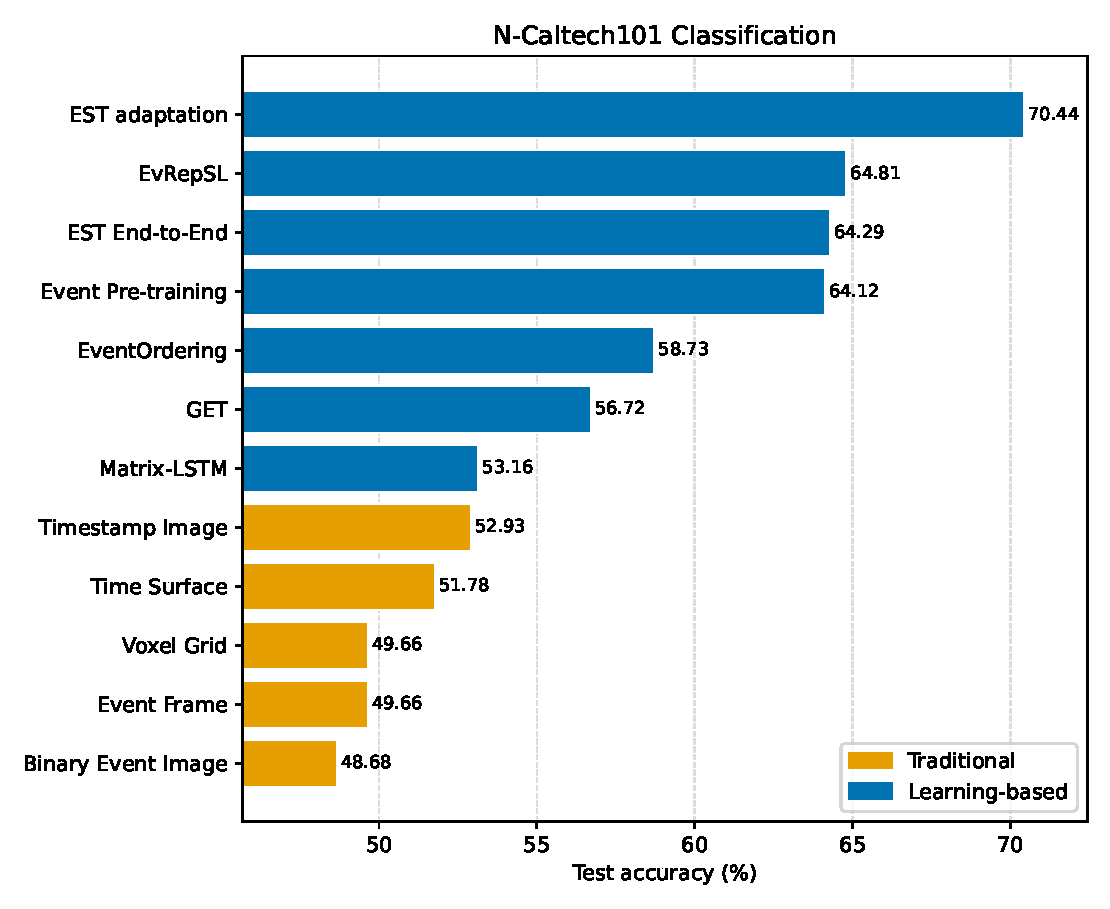
\includegraphics[width=0.92\linewidth]{ncaltech101_accuracy_brief.pdf}
  \caption{N-Caltech101 分类准确率对比。蓝色为 learning-based 方法，橙色为 traditional 方法。N-Caltech101 更复杂，因此更能区分不同事件表示。}
  \label{fig:ncaltech}
\end{figure}

\paragraph{N-Caltech101：Learning-based 优势更明显。} N-Caltech101 的结果与 N-MNIST 明显不同。图 \ref{fig:ncaltech} 显示，Learning-based 方法整体处于更高区间：EST adaptation 达到 70.44\%，EvRepSL 为 64.81\%，EST End-to-End 为 64.29\%，Event Pre-training 为 64.12\%。Traditional 中最好的 Timestamp Image 为 52.93\%，Time Surface 为 51.78\%。因此，在 N-Caltech101 上，best learning-based 与 best traditional 之间约有 17.51 个百分点差距。这个结果说明，在更复杂的分类场景中，学习型表示或学习型 pipeline 能更有效地组织事件流信息；同时也说明 traditional baseline 仍然是必要参照，因为它给出了一个明确的非学习表示下界。

\begin{figure}[t]
  \centering
  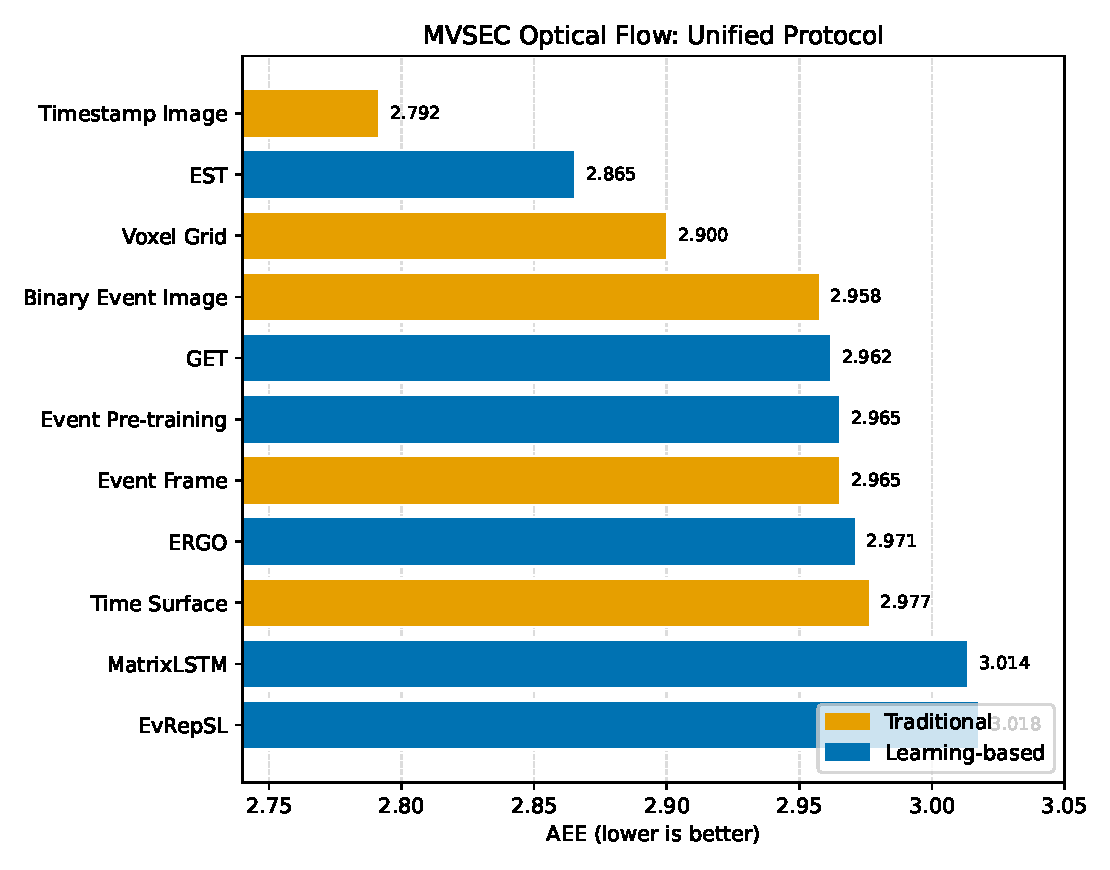
\includegraphics[width=0.88\linewidth]{mvsec_aee_brief.pdf}
  \caption{MVSEC optical flow 统一协议下的 AEE 对比。AEE 越低越好。该图采用局部放大横轴，因为所有方法集中在 2.79 到 3.02 之间。}
  \label{fig:mvsec}
\end{figure}

\paragraph{MVSEC：统一协议下 Traditional 仍具竞争力。} MVSEC 是目前 traditional 和 learning-based 对齐最充分的任务：所有方法使用 outdoor\_day1/2 训练，indoor\_flying1/2/3 测试，窗口大小和 stride 均为 200，并共享 EVFlowNet-like decoder。图 \ref{fig:mvsec} 显示，Timestamp Image 取得最低 AEE 2.7916 和最低 outlier rate 36.61\%，优于当前最好的 learning-based 方法 EST，后者 AEE 为 2.8654，outlier rate 为 37.04\%。Voxel Grid 排名第三，AEE 为 2.9001。这个结果不应被表述为 traditional 方法在原论文设置下全面超过 learning-based 方法，因为这里比较的是统一 benchmark decoder；但它清楚说明，在 optical flow 中，保留 timestamp 信息的传统表示是非常强的 baseline。

\paragraph{汇报结论。} 综合来看，三个任务呈现出不同趋势。N-MNIST 接近饱和，traditional Voxel Grid 和 learning-based EvRepSL 的差距很小；N-Caltech101 更复杂，learning-based 方法明显领先，EST adaptation 比最佳 traditional Timestamp Image 高约 17.51 个百分点；MVSEC 在统一协议下则显示 traditional Timestamp Image 具有很强竞争力，AEE 低于当前 learning-based 最优 EST。因此，晚上汇报时建议采用更稳妥的表述：traditional baseline 在简单分类和光流任务中并不弱，尤其 timestamp-preserving 表示值得重视；但在复杂分类任务 N-Caltech101 上，learning-based 方法优势更清晰。后续工作应继续补齐 N-MNIST 上更多 learning-based 方法，以及 GEN1 detection 的完整对齐结果。

\end{document}
